\mchapter{روش پیشنهادی}
در این فصل الگوریتمی ارائه می‌دهیم که با استفاده از آن می‌توان مسئله‌ی یافتن استراتژی تخلیه با تاخیر کمینه را که در فصل قبل تشریح شد، حل کرد. استراتژی خروجی توسط الگوریتم،‌ از نوع تصادفی می‌باشد و برای بدست آوردن آن، از روشی مبتنی بر زنجیره‌ی مارکوف و برنامه‌ریزی خطی استفاده می‌کنیم.

\section{استراتژی تخلیه‌ی وظیفه‌ی تصادفی}
با استفاده از مدل‌های توصیف شده در فصل قبل می‌توانیم یک تعریف ریاضی از «استراتژی تخلیه وظیفه‌ی تصادفی» داشته باشیم. مشابه با مقاله \Cite{Liu} استراتژی تخلیه‌ی تصادفی را به صورت یک توزیع احتمالی مانند \(g_\tau^a\) بر روی مجموعه‌ی \(S \times A\) تعریف می‌کنیم. در اینجا عبارت \(S \times A\) نمایانگر ضرب دکارتی مجموعه‌ی تمام حالت‌های سیستم در مجموعه‌ی تمام کنش‌های ممکن در سیستم است. یک نکته قابل توجه این است که برخی از دوتایی‌های حاصل از این ضرب دکارتی هیچ‌گاه در واقعیت امکان‌پذیر نیست. برای مثال در حالتی که صف خالی باشد، تنها یک کنش امکان‌پذیر است و آن هم کنش شماره ۱ (\lr{No Operation}) است. با این حال برای سادگی در توضیح روش حل مسئله، این دوتایی‌ها را نیز در دامنه تابع توزیع احتمالی استراتژی تخلیه در نظر می‌گیریم تا همواره تعداد اعضای دامنه‌ی تابع توزیع احتمال برابر با \(|S| \cdot |A|\) باشد. \\

همچنین طبق تعریف توزیع احتمال، رابطه‌ی \ref{eq:prob} باید برای هر استراتژی تخلیه تصادفی برقرار باشد.
\begin{equation}
	\label{eq:prob}
	\sum_{\tau \in S} \sum_{a \in A} g_{\tau}^{a}=1
\end{equation}
\section{مدل زنجیره‌ی مارکوف دستگاه کاربر}
\label{sec:markov}
در این قسمت ابتدا مدل آماری زنجیره‌ی مارکوف گسسته-زمان را معرفی می‌کنیم و سپس توضیح می‌دهیم که چگونه می‌توان با استفاده از این مدل معیارهای تاخیر و توان مصرفی میانگین را برای یک سیستم تخلیه‌ی وظیفه محاسبه کرد.
\begin{defi}
\label{def:one}
دنباله‌ای از متغیرهای تصادفی $X_{1}, X_{2}, \ldots$ را که احتمال تغییر وضعیت از زمان $t$ به $t + 1$ مستقل از وضعیت‌های قبلی باشد را یک \textbf{زنجیره‌ی مارکوف گسسته-زمان} می‌نامند. این گزاره را به بیان متغیرهای تصادفی و تابع احتمال به صورت رابطه‌ی زیر نشان می‌دهیم.
\begin{equation*}
	\operatorname{Pr}\left(X_{t+1}=x \mid X_{1}=x_{1}, X_{2}=x_{2}, \ldots, X_{n}=x_{t}\right)=\operatorname{Pr}\left(X_{t+1}=x \mid X_{t}=x_{t}\right)
\end{equation*}
\end{defi}
زنجیره‌ی مارکوف گسسته‌-زمان را می‌توان با گراف جهت‌دار نیز نمایش داد. در شکل \ref{fig:gambler} یک زنجیره‌ی نمونه مشاهده می‌شود.
\begin{figure}[H]
	\centering
	\begin{latin}
			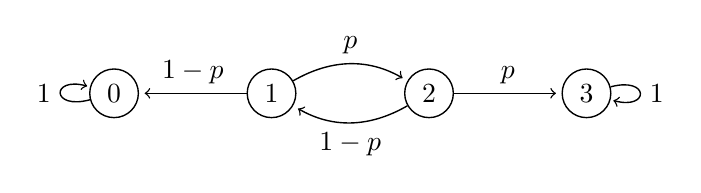
\begin{tikzpicture}[ - > , shorten >=2pt , line width =0.5 pt , node distance =2 cm]
			\node [circle , draw] (zero) {0};
			\node [circle , draw] (one) [right of=zero] {1};
			\node [circle , draw] (two) [right of=one] {2};
			\node [circle , draw] (three) [right of=two] {3};
			\path (zero) edge [loop left] node {$1$} (zero) ;
			\path (one) edge node [above] {$1 - p$} (zero) ;
			\path (one) edge [bend left] node [above]{$p$} (two) ;
			\path (two) edge node [above]{$p$} (three) ;
			\path (two) edge [bend left] node [below]{$1 - p$} (one) ;
			\path (three) edge [loop right] node {$1$} (three) ;
		\end{tikzpicture}
	\end{latin}
	\caption[یک زنجیره‌ی مارکوف نمونه برای مسئله‌ی پاکباختگی]{یک زنجیره‌ی مارکوف نمونه برای مسئله‌ی پاکباختگی قمارباز\protect\footnotemark}
	\label{fig:gambler}
\end{figure}
\LTRfootnotetext{The Gambler's ruin}
\newpage
\begin{defi}
\label{def:two}
زنجیره‌ی مارکوف گسسته-زمان $X(t)$ را \textbf{همگن-زمان} می‌گوییم اگر شرط زیر همواره برقرار باشد:
\begin{equation*}
P\left(X_{n+1}=j \mid X_{n}=i\right)=P\left(X_{1}=j \mid X_{0}=i\right)
\end{equation*}
به عبارت دیگر یعنی احتمالات مربوط به انتقال بین حالت‌ها به زمان \(t\) وابسته نیستند. در این حالت احتمال انتقال زنجیره از حالت \(i\) به \(j\) را با عبارت $p_{i j}=P\left(X_{1}=j \mid X_{0}=i\right)$ نمایش می‌دهیم و همچنین ماتریس انتقال را با $P=\left(p_{i j}\right)$ نمایش می‌دهیم.
\end{defi}
طبق تعاریف \ref{def:one} و \ref{def:two} می‌توان حالت دستگاه کاربر در طی زمان را به صورت یک زنجیره‌ی مارکوف گسسته‌زمان در نظر گرفت به طوری که $\tau[t]$ حالت زنجیره در زمان $t$ را مشخص می‌کند. همچنین ماتریس انتقال $\chi$ را اینگونه تعریف می‌کنیم که $\chi_{\tau, \tau^{\prime}}$ احتمال انتقال از حالت $\tau$ به \(\tau^{\prime}\) را مشخص می‌کند. این ماتریس انتقال به ازای یک استراتژی تخلیه‌ی داده شده و پارامترهای سیستمی مشخص، قابل محاسبه می‌باشد. به طور دقیق‌تر احتمال انتقال از حالتی مانند 
$\tau$
به 
$\tau^\prime$
بستگی به مقادیر زیر دارد:
\begin{itemize}
	\item استراتژی تخلیه $g_\tau^a$
	\item احتمال ورود وظایف $\alpha_1, \cdots, \alpha_k$
	\item احتمال موفقیت واحد ارسال $\beta$
\end{itemize}
برای نمونه در سیستم تخلیه‌ی وظیفه‌ای با ویژگی‌های مشخص شده در جدول \ref{table:fixedranged2} احتمال انتقال به حالات بعدی مطابق با جدول \ref{table:transitions} بدست می‌آید. برای سادگی در اینجا از توضیح بیشتر در مورد نحوه‌ی محاسبه‌ی مقادیر درایه‌های ماتریس انتقال صرف نظر می‌کنیم. برای آگاهی از نحوه‌ی محاسبه‌ی این مقادیر در قالب کد به \hyperref[appendix:3]{پیوست ۳} رجوع شود.
\begin{table}[H]
	\centering
	\begin{latin}
		\begin{tabular}{@{}llllllllllll@{}}
			\toprule
			\textbf{Parameter} & $M_1$ & $M_2$ & $L_1$ & $L_2$ & $C_1$ & $C_2$ & $\beta$ & $P_{tx}$ & $P_{loc}$ & $P_{max}$ & $t_{rx}$ \\ \midrule
			\textbf{Value}     & 1     & 3     & 7     & 2     & 1     & 1     & 0.95    & 1        & 0.8       & 1.6       & 0        \\ \bottomrule
		\end{tabular}
	\end{latin}
	\caption{پارامترهای محیط رایانش لبه‌ای در سناریوی دو صف با یک صف ثابت}
	\label{table:fixedranged2}
\end{table}

\begin{table}[H]
	\centering
	\begin{latin}

\begin{tabular}{|l|l|}
	\hline
	\textbf{$\tau^\prime$}          & \textbf{$\chi_{\tau, \tau^{\prime}}$}                            \\ \hline
$([1,1], 0, 2, 0, 1 )$ & $g_{\tau}^{N o O p e r a t i o n}$ * $(1 - \alpha_1)$ * $(1 - \alpha_2)$             \\ \hline
$([2,1], 0, 2, 0, 1 )$ & $g_{\tau}^{N o O p e r a t i o n}$ * $\alpha_1$ * $(1 - \alpha_2)$              \\ \hline
$([1,2], 0, 2, 0, 1 )$ & $g_{\tau}^{N o O p e r a t i o n}$ * $(1 - \alpha_1)$ * $\alpha_2$              \\ \hline
$([2,2], 0, 2, 0, 1 )$ & $g_{\tau}^{N o O p e r a t i o n}$ * $\alpha_1$ * $\alpha_2$                    \\ \hline
$([0,1], 0, 2, 0, 1 )$ & $g_{\tau}^{A d d T o T U ( 1 )}$ * $\beta$ * $(1 - \alpha_1)$ * $(1 - \alpha_2)$       \\ \hline
$([0,1], 1, 2, 1, 1 )$ & $g_{\tau}^{A d d T o T U ( 1 )}$ * $(1 - \beta)$ * $(1 - \alpha_1)$ * $(1 - \alpha_2)$ \\ \hline
$([1,1], 0, 2, 0, 1 )$ & $g_{\tau}^{A d d T o T U ( 1 )}$ * $\beta$ * $\alpha_1$ * $(1 - \alpha_2)$        \\ \hline
$([1,1], 1, 2, 1, 1 )$ & $g_{\tau}^{A d d T o T U ( 1 )}$ * $(1 - \beta)$ * $\alpha_1$ * $(1 - \alpha_2)$  \\ \hline
$([0,2], 0, 2, 0, 1 )$ & $g_{\tau}^{A d d T o T U ( 1 )}$ * $\beta$ * $(1 - \alpha_1)$ * $\alpha_2$        \\ \hline
$([0,2], 1, 2, 1, 1 )$ & $g_{\tau}^{A d d T o T U ( 1 )}$ * $(1 - \beta)$ * $(1 - \alpha_1)$ * $\alpha_2$  \\ \hline
$([1,2], 0, 2, 0, 1 )$ & $g_{\tau}^{A d d T o T U ( 1 )}$ * $\beta$ * $\alpha_1$ * $\alpha_2$              \\ \hline
$([1,2], 1, 2, 1, 1 )$ & $g_{\tau}^{A d d T o T U ( 1 )}$ * $(1 - \beta)$ * $\alpha_1$ * $\alpha_2$        \\ \hline
$([1,0], 2, 2, 2, 1 )$ & $g_{\tau}^{A d d T o T U ( 2 )}$ * $\beta$ * $(1 - \alpha_1)$ * $(1 - \alpha_2)$       \\ \hline
$([1,0], 1, 2, 2, 1 )$ & $g_{\tau}^{A d d T o T U ( 2 )}$ * $(1 - \beta)$ * $(1 - \alpha_1)$ * $(1 - \alpha_2)$ \\ \hline
$([2,0], 2, 2, 2, 1 )$ & $g_{\tau}^{A d d T o T U ( 2 )}$ * $\beta$ * $\alpha_1$ * $(1 - \alpha_2)$        \\ \hline
$([2,0], 1, 2, 2, 1 )$ & $g_{\tau}^{A d d T o T U ( 2 )}$ * $(1 - \beta)$ * $\alpha_1$ * $(1 - \alpha_2)$  \\ \hline
$([1,1], 2, 2, 2, 1 )$ & $g_{\tau}^{A d d T o T U ( 2 )}$ * $\beta$ * $(1 - \alpha_1)$ * $\alpha_2$        \\ \hline
$([1,1], 1, 2, 2, 1 )$ & $g_{\tau}^{A d d T o T U ( 2 )}$ * $(1 - \beta)$ * $(1 - \alpha_1)$ * $\alpha_2$  \\ \hline
$([2,1], 2, 2, 2, 1 )$ & $g_{\tau}^{A d d T o T U ( 2 )}$ * $\beta$ * $\alpha_1$ * $\alpha_2$              \\ \hline
$([2,1], 1, 2, 2, 1 )$ & $g_{\tau}^{A d d T o T U ( 2 )}$ * $(1 - \beta)$ * $\alpha_1$ * $\alpha_2$        \\ \hline



\end{tabular}
	\end{latin}
\caption[مقادیر ماتریس انتقال]{مقادیر ماتریس انتقال $\chi_{\tau, \tau^{\prime}}$ در صورت حضور در حالت $\tau = ( [1, 1], 0, 1, 0, 1 )$}
	\label{table:transitions}
\end{table}
در نمایش زنجیره‌ی مارکوف به صورت گراف،‌ هر درایه ماتریس انتقال مانند $p_{i, j}$ معادل یک یال جهت‌دار از راس $i$ به راس $j$ با وزن $p_{i, j}$ می‌باشد. بنابراین می‌توان گفت که جدول \ref{table:transitions} یال‌های گراف از راس مبدا $\tau = ( [1, 1], 0, 1, 0, 1 )$ را مشخص می‌کند. در شکل \ref{fig:digraph} گراف جهت‌دار متناظر با سیستم تخلیه‌ی وظیفه‌ی نمونه‌ای رسم شده است که در آن یک صف وظیفه وجود دارد، \(Q = 2\) و هر وظیفه دو قسمت و یک بسته دارد.\footnote{کد استفاده شده برای رسم این گراف در آدرس \lr{https://github.com/dalisyron/OffloadingVisualizer} موجود می‌باشد} با توجه به اینکه تنها یک نوع وظیفه وجود دارد، از متغیرهای $T_L$ و $T_R$ در فضای حالت صرف نظر شده است. در این زنجیره، سه‌تایی $(x, y, z)$ بیانگر حالتی است که در آن $x$ وظیفه در صف وجود دارد، واحد ارسال در وضعیت $y$ قرار دارد و پردازنده $z$ قسمت از وظیفه‌ی تخصیص داده شده به خودش را تاکنون اجرا کرده است.
\begin{landscape}
	\begin{figure}
		\centering
		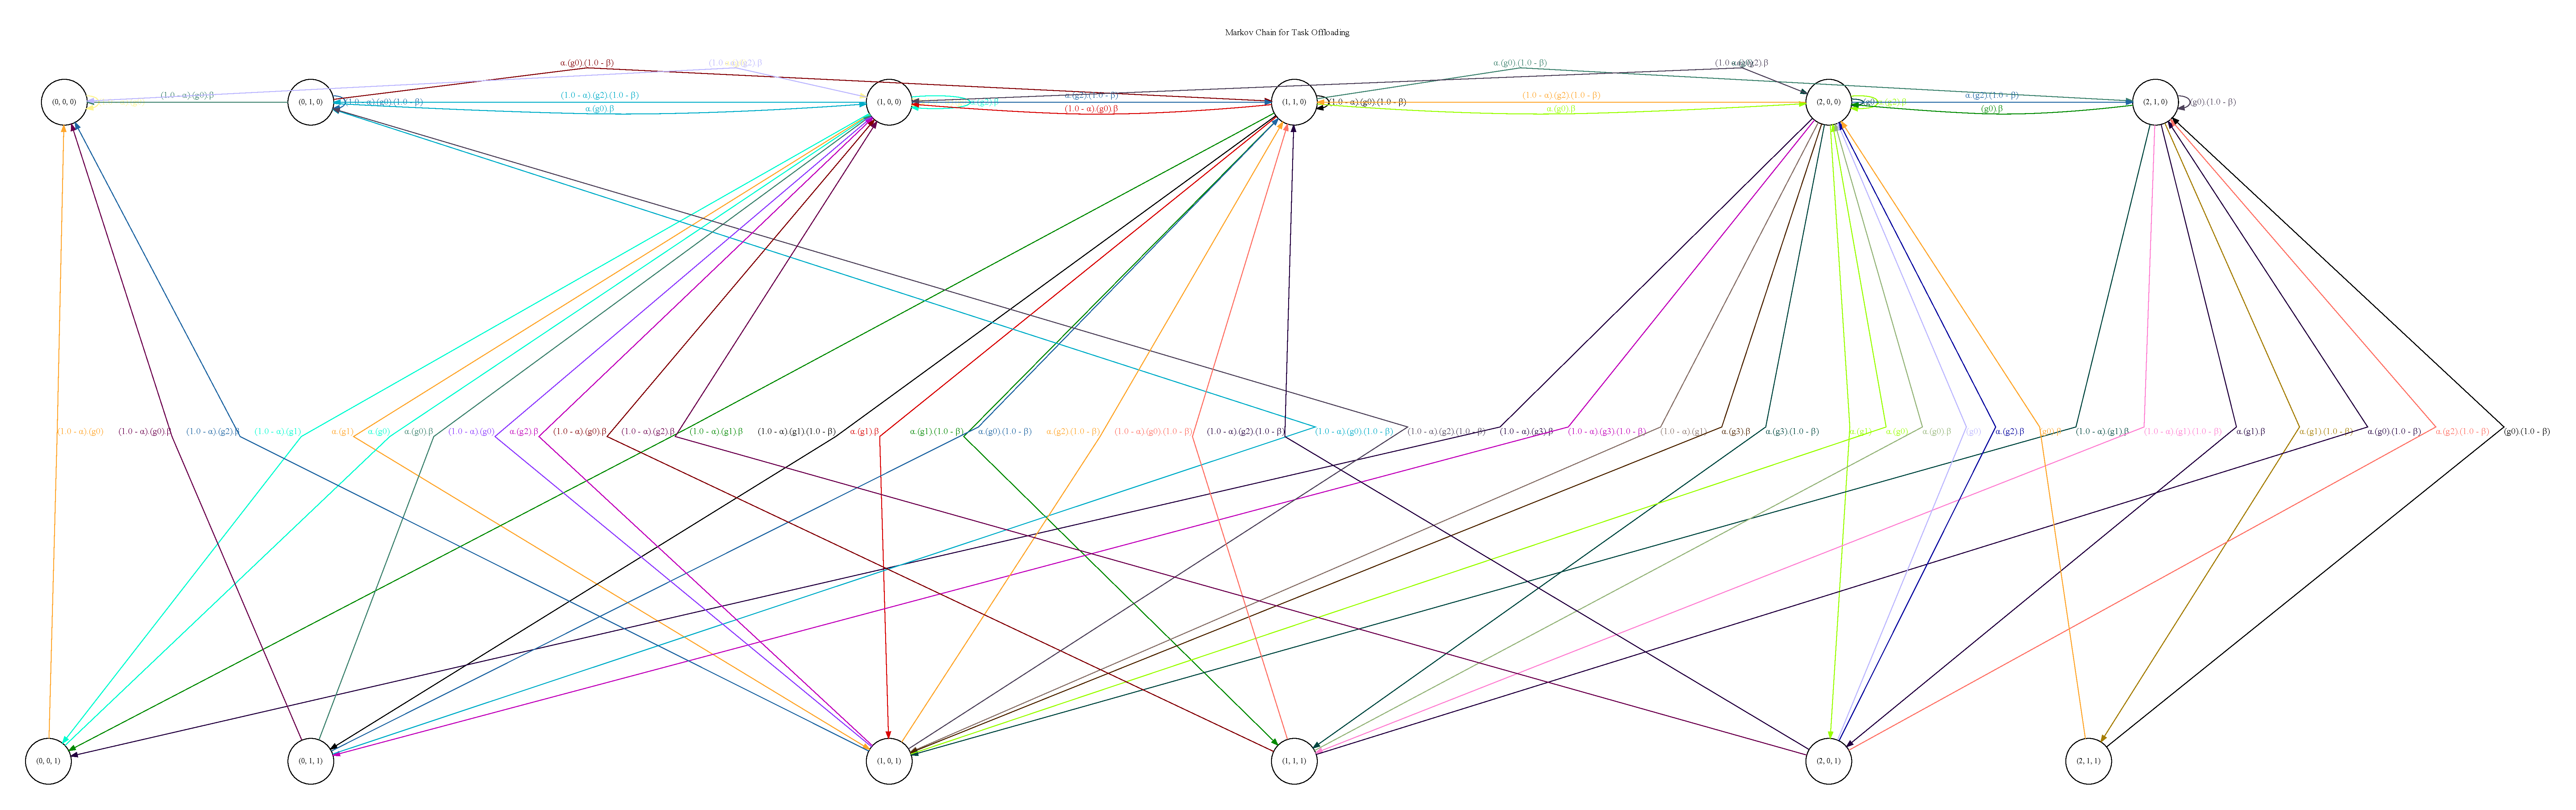
\includegraphics[width=1.5\textwidth]{figures/graph.pdf}
		\caption[زنجیره‌ی مارکوف سیستم تخلیه در قالب گراف جهت‌دار]{
			زنجیره‌ی مارکوف سیستم تخلیه در قالب گراف جهت‌دار (برای مشاهده جزئیات زوم کنید)
		}
		\label{fig:digraph}
	\end{figure}
\end{landscape}
\newpage
\section{محاسبه‌ی تاخیر و توان میانگین با کمک توزیع پایدار}
به منظور محاسبه‌ی معیارهای توان مصرفی میانگین و تاخیر سرویس میانگین لازم است که بتوانیم درباره وضعیت سیستم تخلیه‌ی وظیفه در طولانی‌مدت استنتاج کنیم. در همین راستا مفهوم \textbf{توزیع پایدار} را برای زنجیره‌ی مارکوف تعریف می‌کنیم.
\begin{defi}
توزیع احتمالی مانند $p_i$ را یک \textbf{توزیع پایدار} برای زنجیره‌ی مارکوف با ماتریس انتقال \(P\) می‌گوییم هر گاه شرط زیر در آن برقرار باشد:
\begin{equation*}
	\pi=\pi P \quad \Longleftrightarrow \quad \pi_{j}=\sum_{i} \pi_{i} P_{i j} \quad \forall j .
\end{equation*}
\end{defi}
یک سوالی که ممکن است بوجود بیاید این است که آیا هر زنجیره‌ی مارکوف گسسته‌زمانی توزیع پایدار دارد؟ برای پاسخ به این سوال لازم است دو مفهوم زنجیره‌ی مارکوف تقلیل‌ناپذیر و غیرمتناوب را تعریف کنیم.
\begin{defi}
اگر رسیدن از هر نقطه به نقطه دیگر از فضای حالت با احتمال مثبت در زنجیره‌ی مارکوف میسر باشد، زنجیره را \textbf{تقلیل‌ناپذیر} گویند. به بیان ریاضی می‌توان تقلیل‌ناپذیر بودن زنجیره‌ی مارکوف را به صورت زیر نشان داد.
\begin{equation*}
	\operatorname{Pr}\left(X_{n_{i j}}=j \mid X_{0}=i\right)=p_{i j}^{\left(n_{i j}\right)}>0
\end{equation*}
\end{defi}

\begin{defi}
تناوب $d(i)$ برای حالت $i$ به صورت $d(i)=\operatorname{gcd}\left\{n: P_{i i}^{n}>0\right\}$ تعریف می‌شود، که به معنی بزرگ‌ترین مقسوم علیه مشترک تعداد مراحل ممکن است به صورتی که از $i$ شروع کرده و به $i$ برگردیم. یک زنجیره‌ی مارکوف تقلیل‌ناپذیر را متناوب با تناوب $d$ می‌گوییم اگر تمامی حالت‌ها تناوبی برابر با $d > 1$ را داشته باشند. یک زنجیره‌ی مارکوف تقلیل‌ناپذیر را \textbf{غیرمتناوب} می‌گوییم اگر تمامی حالت‌ها تناوب برابر با ۱ داشته باشند.
\end{defi}
\begin{thm}
\label{thm:converge}
\textbf{(همگرایی)}
هر زنجیره‌ی مارکوف تقلیل‌ناپذیر و غیر متناوب دارای توزیع پایدار منحصر به فردی مانند $\pi$ می‌باشد.
\end{thm}
حال با استفاده از قضیه \ref{thm:converge} ثابت می‌کنیم که زنجیره‌ی مارکوف سیستم تخلیه‌ی وظیفه، دارای توزیع پایدار منحصر به فرد است. برای سادگی فرض می‌کنیم که سامانه یک صف دارد و سپس نحوه‌ی بسط نتیجه به چندین صف را توضیح می‌دهیم.

\begin{thm}
\label{thm:irreducible}
زنجیره‌ی مارکوف مربوط به سیستم تخلیه تک صف تقلیل‌ناپذیر است. \\
\textbf{اثبات:} \\
قسمت الف) با توجه به تعریف سیستم تخلیه می‌دانیم که از هر حالت غیر شروع مانند \( (0, 0, 0) \neq (x, y, z)\) می‌توان به حالت شروع رفت. به این منظور کافی است که تمام وظایف داخل صف به نحوی (اجرا یا ارسال) به اتمام برسند و وظیفه‌ی جدیدی نیز در این حین وارد سیستم نشود. \\

قسمت ب) همچنین می‌توان ثابت کرد که از حالت شروع \((0, 0, 0)\) می‌توان به هر حالت دیگر \((x, y, z)\) رفت. به این منظور دنباله رخدادهای زیر را در نظر بگیرید:
\begin{enumerate}
	\item ورود \(x\) وظیفه‌ی جدید
	\item انتقال یک وظیفه به واحد ارسال و ورود یک وظیفه جدید، هر دو در صورتی که \(y > 0\)
	\item پیشرفت واحد ارسال به مدت \(y\) سیکل و عدم ورود وظیفه‌ی جدید در این حین
	\item انتقال یک وظیفه به پردازنده و ورود یک وظیفه جدید، هر دو در صورتی که \(z > 0\)
	\item پیشرفت واحد ارسال به مدت \(z\) سیکل و عدم ورود وظیفه‌ی جدید در این حین
\end{enumerate}
با توجه به نتایج بخش الف و ب می‌توان نتیجه گرفت که از گشتی با احتمال مثبت از هر حالت به حالت دیگر وجود دارد بنابراین طبق تعریف زنجیره تقلیل‌ناپذیر است.
\end{thm}
\begin{thm}
\label{thm:aperiodic}
زنجیره‌ی مارکوف مربوط به سیستم تخلیه تک صف غیر متناوب است. \\
\textbf{اثبات:} \\
به منظور اثبات این قضیه فقط کافی است که به این نکته توجه کنیم که حالت \((0, 0, 0)\) دارای تناوب یک می‌باشد زیرا با احتمالی مثبت (متناظر با رخداد عدم ورود وظیفه و کنش \lr{No Operation}) می‌توان در همان حالت ماند. با توجه به همین نکته و تقلیل‌ناپذیر بودن زنجیره میتوانیم نتیجه بگیریم که سایر حالت‌ها نیز باید تناوب یک داشته باشند. بنابراین زنجیره غیرمتناوب است.
\end{thm}
با توجه به قضایای \ref{thm:irreducible} و \ref{thm:aperiodic} و قضیه همگرایی می‌توان نتیجه گرفت که زنجیره‌ی مارکوف سیستم تخلیه تک صف دارای توزیع پایدار منحصر به فرد می‌ مطابق با رابطه‌ی \ref{eq:steady} می‌باشد. برای بسط این اثبات به حالت چند صف اثبات غیرمتناوب بودن یکسان خواهد بود و در اثبات تقلیل‌ناپذیر بودن، رخداد اول به ورود \(x_1, \cdots, x_k\) وظیفه از انواع مختلف تغییر پیدا می‌کند.
\begin{equation}
	\label{eq:steady}
	\left\{\begin{array}{l}
		\sum_{\boldsymbol{\tau}^{\prime} \in \mathcal{S}} \chi_{\boldsymbol{\tau}^{\prime}, \boldsymbol{\tau}} \pi_{\boldsymbol{\tau}^{\prime}}=\pi_{\boldsymbol{\tau}}, \forall \boldsymbol{\tau} \in \mathcal{S} \\
		\sum_{\boldsymbol{\tau} \in \mathcal{S}} \pi_{\boldsymbol{\tau}}=1
	\end{array}\right.
\end{equation}
\section{محاسبه‌ی تاخیر میانگین}
تاخیر هر وظیفه، شامل تاخیر انتظار در صف وظایف و تاخیر پردازش می‌باشد. به منظور بدست آوردن تاخیر میانگین سیستم ابتدا $\theta_i$ را به عنوان کسری از وظایف سیستم در طولانی مدت که از نوع $i$ هستند تعریف می‌کنیم. اگر طول صف‌ها به مقدار کافی بزرگ باشد و همچنین استراتژی تخلیه‌ای داشته باشیم که منجر به پر شدن صف و اتلاف وظیفه\LTRfootnote{Task Loss} نشود مقدار $\theta_i$ طبق رابطه‌ی \ref{eq:theta} بدست می‌آید.
\begin{equation}
\label{eq:theta}
\theta_i = \frac{\alpha_i}{\sum_{j=1}^{k} \alpha_{j}}
\end{equation}
\newpage
پارامتر \(t_q^i\) را برابر با مقدار میانگین تاخیر انتظار در صف مربوط به وظایف نوع $i$ تعریف می‌کنیم. طبق قانون لیتِل\LTRfootnote{Little's Law} می‌توان مقدار این تاخیر را بر اساس رابطه‌ی \ref{eq:queuing-delay} بدست آورد. همانطور که پیش‌تر ذکر شد برای برقراری این رابطه لازم است که اتلاف وظیفه در صف رخ ندهد. به عبارت دیگر فقط با فرض اینکه استراتژی تخلیه‌ی ارائه‌شده «کارامد» باشد رابطه‌ \ref{eq:queuing-delay} برقرار است. در پیاده‌سازی عملی، محدودیت «کارآمد» بودن یک استراتژی بدین گونه تعریف شده است که احتمال پر بودن صف مقداری ناچیز باشد.

\begin{equation}
	\label{eq:queuing-delay}
	t_{q}^i=\frac{\theta_i}{\alpha_i} \sum_{j=0}^{Q} i \cdot \operatorname{Pr}\{q_i[t]=i\}=\frac{1}{\alpha} \sum_{\tau \in S} \tau\{q_i\} \cdot \pi_{\tau}
\end{equation}
همچنین $t_{tx}^i$ را به عنوان تاخیر ارسال میانگین یک وظیفه از نوع \(i\) توسط واحد ارسال تعریف می‌کنیم که مقدار آن بر اساس امید ریاضی موفقیت در فرآیند برنولی مطابق با رابطه‌ی \ref{eq:bernouli} بدست می‌آید.
\begin{equation}
	\label{eq:bernouli}
	t_{t x}^i=M_i \sum_{j=1}^{\infty} j(1-\beta)^{(j-1)} \beta
\end{equation}
به یاد داریم که مقدار تاخیر در صورت پردازش محلی برای وظایف نوع $i$ برابر $L_i$ می‌باشد. تاخیر اجرا در صورت تخلیه‌ی وظیفه به صورت مجموع زمان ارسال وظیفه
$t_{tx}^i$
زمان اجرا در سرور لبه‌ای
$C_i$
و تاخیر دریافت نتیجه از سرور
$t_{rx}^i$
محاسبه می‌شود.
\begin{equation}
	t_{c}^i=t_{t x}^i+C_i+t_{rx}
\end{equation}
در نتیجه می‌توان تاخیر اجرای میانگین وظایف نوع $i$ را نیز مطابق رابطه‌ی \ref{eq:proc-delay} بیان کرد.
\begin{equation}
	\label{eq:proc-delay}
	t_{p}^i=\eta_i L_i+(1-\eta_i) t_{c}^i
\end{equation}
که در آن
$\eta_i$
بیانگر کسری از وظایف نوع $i$ می‌باشد که در طولانی‌مدت به صورت محلی اجرا می‌شوند و مطابق با رابطه‌ی \ref{eq:eta} بدست می‌آيد.
\begin{equation}
	\label{eq:eta}
	\eta_i=\frac{\sum_{\boldsymbol{\tau, a} \in \mathcal{S}_{1}^i\cup\mathcal{S}_{3}^i\cup\mathcal{S}_{5}^i} \pi_{\boldsymbol{\tau}} g_{\boldsymbol{\tau}}^{a} }{\sum_{\boldsymbol{\tau, a} \in \mathcal{S}_{1}^i\cup\mathcal{S}_{2}^i\cup\mathcal{S}_{3}^i\cup\mathcal{S}_{4}^i} \pi_{\boldsymbol{\tau}} g_{\boldsymbol{\tau}}^{a} + 2 \sum_{\boldsymbol{\tau, a} \in S_5^i} \pi_{\boldsymbol{\tau}} g_{\boldsymbol{\tau}}^{a}}
\end{equation}
که در آن
$S_1^i, \cdots, S_5^i$
به صورت زیر تعریف می‌شوند:
\begin{equation}
	\begin{aligned}
		& S_1^i = \{\boldsymbol{\tau, a} \in \mathcal{S} \times A | type(a) = AddToCPU \land cpuQueue(a) = i\} \\
		& S_2^i = \{\boldsymbol{\tau, a} \in \mathcal{S} \times A | type(a) = AddToTU \land tuQueue(a) = i\} \\ 
		& S_3^i = \{\boldsymbol{\tau, a} \in \mathcal{S} \times A | type(a) = AddToBoth \land cpuQueue(a) = i \land tuQueue(a) \neq i\} \\
		& S_4^i = \{\boldsymbol{\tau, a} \in \mathcal{S} \times A | type(a) = AddToBoth \land cpuQueue(a) \neq i \land tuQueue(a) = i\} \\
		& S_5^i = \{\boldsymbol{\tau, a} \in \mathcal{S} \times A | type(a) = AddToBoth \land cpuQueue(a) = i \land tuQueue(a) = i\}
	\end{aligned}
\end{equation}
در رابطه‌ی فوق تابع $type(a)$ نوع کنش را مشخص می‌کند و یکی از چهار نوع بیان شده در بخش \ref{sec:action} می‌باشد. توابع
$cpuQueue(a)$
و
$tuQueue(a)$
نیز نوع وظیفه‌ی مربوط به کنش $a$ را مشخص می‌کنند. \\

با استفاده از روابط بالا همچنین می‌توانیم میانگین تاخیر سرویس هر وظیفه در سیستم را طبق رابطه‌ی \ref{eq:total-delay} محاسبه کنیم. رابطه‌ی بدست آمده برای $\bar{T}$ همچنین مشخص کننده تابع هدف در مسئله‌ی پیدا کردن استراتژی تخلیه‌ی بهینه می‌باشد.
\begin{equation}
	\label{eq:total-delay}
	\bar{T}=\sum_{i=1}^{k} \theta_{i}\left(t_{q}^{i}+t_{p}^{i}\right)
\end{equation}
\newpage
\section{توان مصرفی میانگین}
اگر پارامتر
$\mu_\tau^{loc}$
و 
$\mu_\tau^{tx}$
را به ترتیب به عنوان احتمال فعالیت پردازنده در حالت
$\tau$
و احتمال وجود درخواست ارسال وظیفه در حالت
$\tau$
تعریف کنیم، و $v_{loc}$ و $v_{tx}$ را به صورت مجموع این دو پارامتر در فضای حالت مسئله تعریف کنیم، آنگاه توان مصرفی میانگین طبق رابطه‌ی زیر بدست می‌آید:
\begin{equation}
	\begin{aligned}
		\bar{P} &=\sum_{\boldsymbol{\tau} \in \mathcal{S}} \pi_{\boldsymbol{\tau}}\left(\mu_{\boldsymbol{\tau}}^{l o c} P_{l o c}+\beta \mu_{\boldsymbol{\tau}}^{t x} P_{t x}\right) \\
		&= \sum_{\boldsymbol{\tau} \in \mathcal{S}} \pi_{\boldsymbol{\tau}}\left(\mu_{\boldsymbol{\tau}}^{l o c} P_{l o c}\right) + \sum_{\boldsymbol{\tau} \in \mathcal{S}} \pi_{\boldsymbol{\tau}}\left(\beta\mu_{\boldsymbol{\tau}}^{t x} P_{t x}\right) \\
		&=v_{loc}P_{loc} + \beta v_{tx}P_{tx}
	\end{aligned}
\end{equation}
در اینجا فرض می‌کنیم که مقادیر $\mu_\tau^{loc}$ و $\mu_\tau^{tx}$ از قبل معلوم است. در \hyperref[appendix:2]{پیوست ۲} نحوه‌ی بدست آوردن مقادیر $v_{tx}$ و $v_{loc}$ در قالب کد شرح داده شده است.
\section{استراتژی تخلیه‌ی وظیفه‌ی بهینه}
\label{sec:strat}
با توجه به توابع بدست آمده برای تاخیر و توان مصرفی میانگین در بخش‌های پیشین، حال می‌توانیم مسئله‌ی پیدا کردن استراتژی تخلیه‌ی بهینه را به صورت یک مسئله‌ی بهینه سازی مانند
$\mathcal{P}_{1}$
بیان کنیم:
\begin{equation}
		\begin{aligned}
			\mathcal{P}_{1}: \min _{\left\{g_{\tau}^{a}\right\}}\; & \bar{T} = (\sum_{i=1}^{k} \frac{1}{\alpha_i} \sum_{\tau \in S} \tau\{q_i\} \cdot \pi_{\tau}) + T_p^0 \\
			\text { \lr{s.t.} } &\left\{\begin{array}{l}
				\bar{P} \leq \bar{P}_{\max } \\
				\sum_{\boldsymbol{\tau}^{\prime} \in \mathcal{S}} \chi_{\boldsymbol{\tau}^{\prime}, \boldsymbol{\tau}} \pi_{\boldsymbol{\tau}^{\prime}}=\pi_{\boldsymbol{\tau}}, \boldsymbol{\tau} \in \mathcal{S}, \\
				\sum_{\boldsymbol{\tau} \in S} \pi_{\boldsymbol{\tau}}=1, \\
				\sum_{\alpha \in A} g_{\tau}^{\alpha}=1, \forall \tau \in S\\
				g_{\tau}^{a} \geq 0, \forall \tau \in S,\;a \in A
			\end{array}\right.
		\end{aligned}
\end{equation}
که در آن
$T_p^0$
برابر با تاخیر اجرای میانگین است که به ازای مقادیر داده شده از
$\eta_0, \cdots, \eta_k$
مقداری ثابت دارد و از رابطه‌ی زیر بدست می‌آید:
\begin{equation}
	T_p^0 = \sum_{i=1}^{k} (\eta_i L_i+(1-\eta_i) t_{c}^i)
\end{equation}
مسئله‌ی
$\mathcal{P}_{1}$
به دلیل وجود پارامتر $\eta_i$ در تابع هدف یک مسئله خطی نیست. با این حال می‌توانیم با استفاده از تغییری کوچک مسئله را به مجموعه‌ای از مسائل برنامه‌ریزی خطی تبدیل کنیم. به این منظور مشابه با \Cite{Liu} ابتدا از تعریف «معیار احاطه\LTRfootnote{Occupation Measure}» در زنجیره‌ی مارکوف استفاده می کنیم. به این منظور مجموعه متغیرهای جایگزین $\left\{x_{\tau}^{a}\right\}$ را طبق رابطه‌ی $x_{\tau}^{a}=\pi_{\tau} g_{\tau}^{a}$ تعریف می‌کنیم. به عبارتی $x_{\tau}^{a}$ برابر با احتمال حضور در حالت $\tau$ و انتخاب کنش
$a$
می‌باشد. همچنین طبق تعریف می‌دانیم که
$\sum_{a \in A} g_{\tau}^{a}=1$
بنابراین خواهیم داشت
$\pi_{\boldsymbol{\tau}}=\sum_{a \in A} x_{\boldsymbol{\tau}}^{a}$
\\\\
حال با جایگذاری $\left\{x_{\tau}^{a}\right\}$ به جای $\{\pi_\tau\}$ در
$\mathcal{P}_{1}$
خواهیم داشت:
\begin{equation}
	\label{eq:p2}
	\begin{aligned}
		\mathcal{P}_{2}: \min _{\boldsymbol{x}, \eta}\; & \bar{T}=(\sum_{i=1}^{k} \frac{1}{\alpha_i} \sum_{\tau \in \mathcal{S}} \sum_{a \in A} \tau\{q_i\} \cdot x_{\tau}^{a})+ T_p^0 \\
		\text { \lr{s.t.} } &\left\{\begin{array}{l}
			\nu_{l o c}(\boldsymbol{x}) P_{l o c}+\beta \nu_{t x}(\boldsymbol{x}) P_{t x} \leq \bar{P}_{\max } \\
			\Gamma(\boldsymbol{x}, \eta_i)=, \forall i \in \{1, \cdots, k\}\\
			F_{\tau}(\boldsymbol{x})=0, \forall \tau=(i, m, n) \in \mathcal{S} \\
			\sum_{\tau \in \mathcal{S}} \sum_{a \in A}=1 \\
			\eta_i \in [0, 1], \forall i \in \{1, \cdots, k\} \\
			x_{\tau}^{a} \geq 0, \forall \tau \in S, a \in A
		\end{array}\right.
	\end{aligned}
\end{equation}
که در آن
$\nu_{l o c}$
و
$\nu_{t x}$
به ترتیب احتمال فعالیت پردازنده و واحد ارسال را در یک واحد زمانی دلخواه مشخص می‌کنند و به ازای یک استراتژی داده شده قابل محاسبه اند. \footnote{برای مشاهده روش محاسبه این دو پارامتر در قالب کد به پیوست ۲ مراجعه شود.} تابع
$\Gamma(\boldsymbol{x}, \eta_i)$
بر اساس رابطه‌ی \ref{eq:eta} می‌باشد و به صورت زیر محاسبه می‌شود:
\begin{equation}
	\Gamma(x, \eta) = \eta  \sum_{\boldsymbol{\tau, a} \in \mathcal{S}_{1}^i\cup\mathcal{S}_{2}^i\cup\mathcal{S}_{3}^i\cup\mathcal{S}_{4}^i} x_{\tau}^a + 2 \eta \sum_{\boldsymbol{\tau, a} \in S_5^i} x_{\tau}^a
	- \eta \sum_{\boldsymbol{\tau, a} \in \mathcal{S}_{1}^i\cup\mathcal{S}_{3}^i\cup\mathcal{S}_{5}^i} x_{\tau}^a
\end{equation}
و تابع 
$F_{\tau}(\boldsymbol{x})$
به صورت زیر تعریف می‌شود:
\begin{equation}
	F_{\tau}(\boldsymbol{x})=\sum_{\tau^{\prime} \in \mathcal{S}} \sum_{a \in A} \tilde{\chi}_{\tau^{\prime}, \tau, a} x_{\tau^{\prime}}^{a}-\sum_{a \in A} x_{\tau}^{a}
\end{equation}
در رابطه‌ی فوق منظور از
$\tilde{\chi}_{\tau^{\prime}, \tau, a}$
احتمال شرطی این است که به شرط اینکه در حالت
$\tau^{\prime}$
باشیم و کنش
$a$
انتخاب شده باشد، آنگاه به حالت
$\tau^{\prime}$
برویم و مطابق با رابطه‌ی \ref{eq:conditional} بدست می آید. لازم به ذکر است که مقدار 
$ \tilde{\chi}_{\tau^{\prime}, \tau, a}$ 
بر خلاف 
$\chi_{\tau, \tau^{\prime}}$
نسبت به استراتژی تخلیه احتمالی $g_\tau^a$ مستقل است.
\begin{equation}
	\label{eq:conditional}
	\tilde{\chi}_{\tau, \tau^{\prime}, \alpha}=P\left(\tau[t+1]=\tau^{\prime} \mid \tau[t]=\tau \; \land v[t]=a\right)
\end{equation}

در صورتی که مقادیر
$\eta_0, \cdots, \eta_k$
معلوم باشد آنگاه مسئله
$\mathcal{P}_2$
تبدیل به یک مسئله‌ی برنامه‌ریزی خطی می‌شود. با یافتن مقادیر جواب بهینه
$\left\{x_{\tau}^{a}\right\}$ 
می‌توان استراتژی بهینه را طبق رابطه‌ی زیر بدست آورد:
\begin{equation}
	g_{\tau}^{a *}=\frac{x_{\tau}^{a *}}{\sum_{a \in A} x_{\tau}^{a *}}, \forall \tau \in \mathcal{S}, a \in A
\end{equation}
بنابراین جهت یافتن استراتژی بهینه برای یک سیستم تخلیه‌ی وظیفه کافی است که مسئله‌ی برنامه‌ریزی خطی حاصل از
$\mathcal{P}_2$
را به ازای مقادیر مختلف 
$\eta_0, \cdots, \eta_k$
حل کرده تا استراتژی بهینه بدست بیاید. مراحل این فرآیند جستجو در الگوریتم ۱ به صورت خلاصه آمده است. در این الگوریتم تابع $splitRange$ تابعی است که با گرفتن یک بازه از اعداد حقیقی مانند $R$ و پارامتر $precision$، تعداد $precision$ نمونه با فاصله‌های یکسان از بازه $R$ را در قالب یک لیست بر می‌گرداند. منظور از $splitRange([0, 1], precision)^k$ نیز ضرب دکارتی $k$ نمونه از این لیست‌های خروجی در یک دیگر می‌باشد.

\begin{latin}
	\begin{algorithm}
		\rl{\caption{الگوریتم جستجوی استراتژی تخلیه‌ی وظیفه‌ی بهینه}\label{alg:cap}}
		\begin{algorithmic}[1]
			\Require $precision \geq 2$
			\State $etaSettings \gets splitRange([0, 1], precision)^k$
			\State $optimalPolicy = null$
		    \ForEach {$s \in etaSettings$}
				\State $(\eta_0, \cdots, \eta_k) \gets s$
				\State $solution \gets solveLP(\eta_0, \cdots, \eta_k)$
				\If{$optimalPolicy = null\;\mathbf{or}\;solution.delay < optimalPolicy.delay$}
					\State $optimalPolicy \gets solution.policy$
				\EndIf
			\EndFor \\
			\Return $optimalPolicy$
		\end{algorithmic}
	\end{algorithm}
\end{latin}
\newpage
\section{دو بهینه‌سازی برای الگوریتم جستجوی استراتژی}
\label{sec:optim}
در این بخش دو بهینه‌سازی مختلف را به منظور بهبود عملکرد الگوریتم \ref{alg:cap} معرفی می‌کنیم. این دو بهینه‌سازی در چارچوب \lr{Kompute} که در فصل پیش رو ارائه خواهد شد پیاده‌سازی شده‌اند.
\subsection{کاهش تعداد متغیرها}
\label{sub:reducevariable}
در مسئله‌ی بهینه‌سازی 
$\mathcal{P}_2$
تعداد 
$|S| \cdot |A|$
متغیر وجود دارد. این مقدار برای تعداد صف‌های کم (برای مثال $k \leq 3$) قابل اجرا می‌باشد اما با افزایش تعداد صف‌ها اجرای الگوریتم را بسیار زمان‌بر و یا غیرممکن می‌کند. یک بهینه‌سازی خیلی ساده ولی کارآمد که در \Cite{Liu} به آن اشاره‌ای نشده است این است که می‌توان تمام متغیرهای مانند
$x_{\tau}^{a}$
که کنش
$a$
جزو کنش‌های ممکن در
$\tau$
نباشد را حذف کرد زیرا مقدار آنها در جواب مسئله‌ی همواره برابر صفر می‌باشد. برای مثال در جدول \ref{table:isactionpossible} مجموعه‌ی تمام کنش‌های سیستم تخلیه توصیف شده در جدول \ref{table:fixedranged2} به همراه امکان‌پذیری هر کنش در صورت حضور در حالت 
$\tau = ([3, 0], 0, 1, 0, 1)$
مشخص شده است.
\begin{table}
	\centering
	\begin{latin}
\begin{tabular}{llc}
	\hline Row & Action & Is Possible \\
	\hline 
1            & \texttt{\footnotesize NoOperation}                                         & Yes \\
2            & \texttt{\footnotesize AddToCPU(queueIndex = 1)}                            & No \\
3            & \texttt{\footnotesize AddToCPU(queueIndex = 2)}                            & No \\
4            & \texttt{\footnotesize AddToTransmissionUnit(queueIndex = 1)}               & Yes \\
5            & \texttt{\footnotesize AddToTransmissionUnit(queueIndex = 2)}               & No \\
6            & \texttt{\footnotesize AddToBothUnits(cpuQueueIndex = 1, tuQueueIndex = 1)} & No  \\
7            & \texttt{\footnotesize AddToBothUnits(cpuQueueIndex = 1, tuQueueIndex = 2)} & No \\
8            & \texttt{\footnotesize AddToBothUnits(cpuQueueIndex = 2, tuQueueIndex = 1)} &No \\
9            & \texttt{\footnotesize AddToBothUnits(cpuQueueIndex = 2, tuQueueIndex = 2)} &No \\\bottomrule
	\hline
\end{tabular}
	\end{latin}
	\caption[امکان‌پذیری کنش‌های مختلف]{امکان‌پذیری کنش‌های مختلف در حالت $\tau = ([3, 0], 0, 1, 0, 1)$}
	\label{table:isactionpossible}
\end{table}
همانطور که مشاهده می‌شود در این حالت فقط ۲ کنش از مجموعه‌ی ۹ کنش موجود در $A$ امکان‌پذیر می‌باشند. کنش‌های ردیف ۲ و ۳ به دلیل مشغول بودن پردازنده امکان‌پذیر نمی‌باشند. کنش ردیف ۵ به دلیل خالی بودن صف وظایف نوع ۲ امکان‌پذیر نمی‌باشد. کنش‌های ردیف ۶ الی ۹ نیز به دلیل مشغول بودن پردازنده امکان‌پذیر نمی‌باشند. بنابراین می‌توانیم به سادگی ۷ متغیر متناظر این کنش‌ها را از مجموعه $\left\{x_{\tau}^{a}\right\}$ حذف کنیم بدون اینکه تغییری در جواب مسئله‌ی بهینه‌سازی $\mathcal{P}_2$ ایجاد شود.
\subsection{موازی‌سازی}
الگوریتم \ref{alg:cap} به گونه‌ای تعریف شده است که امکان موازی‌سازی و مقیاس‌پذیری آن به صورت خطی وجود دارد. به عبارت دیگر می‌توان مسئله‌ی برنامه‌ریزی خطی متناظر با هر مقداردهی از
$\eta_0, \cdots, \eta_k$
را به یک هسته یا گره پردازشی خاص اختصاص داد. در شبیه‌سازی سناریوی وظایف سبک و سنگین (رجوع شود به \ref{sub:heavylight}) مشاهده شد که الگوریتم موازی‌سازی شده هنگام اجرا بر روی سروری با ۲۴ هسته و تقسیم‌بندی به ۲۴ ریسمان عملکردی معادل ۲۰ برابر سریع‌تر از حالت تک‌ریسمان\LTRfootnote{Single-thread} دارد.

\begin{latin}
	\begin{algorithm}
		\rl{\caption{الگوریتم موازی‌سازی شده‌ی جستجوی استراتژی تخلیه‌ی بهینه}\label{alg:conc}}
		\begin{algorithmic}[1]
			\Require $precision \geq 2$
			\Require $threadCnt \geq 1$
			\State \textbf{synchronized} $optimalPolicy = null$
			\Procedure{$findOptimalForEtaSettings$}{$etaSettings$}
			\ForEach {$s \in etaSettings$}
			\State $(\eta_0, \cdots, \eta_k) \gets s$
			\State $solution \gets solveLP(\eta_0, \cdots, \eta_k)$
			\If{$optimalPolicy = null\;\mathbf{or}\;solution.delay < optimalPolicy.delay$}
			\State $optimalPolicy \gets solution.policy$
			\EndIf
			\EndFor
			\EndProcedure
			\State $etaSettings \gets splitRange([0, 1], precision)^k$
			\State $etaBatches \gets splitToBatches(etaSettings, threadCnt)$
			\ForEach {$i \in 1 \cdots threadCnt$}
			\State \(thread[i] = Thread\{findOptimalForEtaSettings(etaBatches[i])\}\)
			\EndFor
			\ForEach {$i \in 1 \cdots threadCnt$}
			\State $thread[i].start()$
			\EndFor
			\ForEach {$i \in 1 \cdots threadCnt$}
			\State $thread[i].join()$
			\EndFor \\
			\Return $optimalPolicy$
		\end{algorithmic}
	\end{algorithm}
\end{latin}